\documentclass[tikz]{standalone}

\input{../../scripts/latex/figure-preamble.tex}


\begin{document}
\scriptsize

\begin{tikzpicture}[anchor=north west]
\filldraw[white] (0,0) rectangle +(18,-0.1);

\begin{scope}[xshift=5cm]
	\node[anchor = north west] at (1.3,-0.2) {
		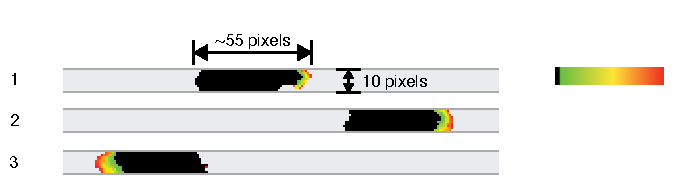
\includegraphics{../cartoons/microchannel-setup.pdf}
	};
	\node[anchor = north west] at (0,0) {\figf B};
	\node[anchor = north west] at (10.7,-1) {Activity:};
	\node[anchor = north west] at (10.7,-1.8) {0};
	\node[anchor = north west] at (11.75,-1.8) {max\textsubscript{act}};
	%\draw (14.1,-0.6 ) rectangle +(5.6,-2.7);
	\filldraw[white] (1.3,-0.2) rectangle +(0.5,-3);
	\node[anchor=north east] at (1.7,-0.9) { $\lambda$/max\textsubscript{act}:};
	\node[anchor=north east] at (1.7,-1.45) {200/30};
	\node[anchor=north east] at (1.7,-2.1) {300/30};
	\node[anchor=north east] at (1.7,-2.8) {200/40};
\end{scope}


\begin{scope}%[xshift=13cm]
	\begin{scope}[xshift=-0.3cm]
	\begin{scope}
		\clip (2.65,-1) rectangle +(2,-2.5);
		\node[anchor = north east, scale=0.5] at (4.75,-1.25) {
			\includegraphics{../example-img/1D-m30l200-1.png}
		};	
		\node[anchor = north east, scale=0.5] at (4.75,-1.98) {
			\includegraphics{../example-img/1D-m30l200-2.png}	
		};
		\node[anchor = north east, scale=0.5] at (4.7,-2.65) {
			\includegraphics{../example-img/1D-m30l200-3.png}	
		};	
	\end{scope}
	
	\draw[->] (0.9,-1.47) -- +(0,-1.8);
	
	\node[anchor = north west, align=left] at (2.65,-0.5) {
		$\lambda$\textsubscript{act} = 200,\\max\textsubscript{act} = 30:
	};
	\node[anchor = north west] at (1,-1.47) {"Go" ($\rightarrow$)};
	\node[anchor = north west] at (1,-2.15) {"Stop"};
	\node[anchor = north west] at (1,-2.85) {"Go" ($\leftarrow$)};
	\end{scope}

	\node[anchor = north west] at (0,0) {\figf A};
\end{scope}

\end{tikzpicture}


\end{document}